\documentclass{mwhittaker}

\usepackage{algorithm}
\usepackage{algpseudocode}
\usepackage{bm}
\usepackage{colors}
\usepackage{enumerate}
\usepackage{environ}
\usepackage{etoolbox}
\usepackage{iconfluence}
\usepackage{ifthen}
\usepackage{mathpartir}
\usepackage{pervasives}
\usepackage{subcaption}
\usepackage{tikz}
\usetikzlibrary{calc}

\newtoggle{showproofs}
\toggletrue{showproofs}
% \togglefalse{showproofs}
\NewEnviron{elidableproof}{%
  \begin{proof}
    \iftoggle%
      {showproofs}
      {\BODY}
      {This proof is elided; toggle \texttt{showproofs} to show the proof.}
  \end{proof}
}

\begin{document}
  \begin{center}
    {\huge \textbf{Invariant-Confluence}} \\
    {\today{}}
  \end{center}

  {\section{\Iconfluence{}}
In this section, we present six different ways to think about \Iconfluence{}:
three state-based approaches and three operation-based approaches.

\subsection{State-Based}
\begin{definition}
  A \defword{distributed state-based object} is a triple $(S, s_0, \join)$
  where $S$ is a set of states, $s_0 \in S$ is a designated start state, and
  $\join: S \times S \to S$ is a binary merge operator that we call join.
\end{definition}

The notion of state-based objects is taken from~\cite{shapiro2011conflict}.
Note that $\join$ is an \emph{arbitrary} function. It does not necessarily have
to satisfy any special properties like associativity or commutativity, though
later we will see that often it does.

\begin{definition}
  A \defword{state-based transaction} $t: S \to S$ is a function that maps one
  state to another.
\end{definition}

\begin{definition}
  An \defword{invariant} $I \subseteq S$ is a subset of states. Notationally,
  we say $I(s)$ to mean $s \in I$ and $\lnot I(s)$ to mean $s \notin I$.
\end{definition}

\begin{example}
  $(\nats, 0, +)$ is a distributed object, $t(x) = 2x$ is a transaction, and
  $\setst{x \in \nats}{x \equiv 0 \mod 2}$ is an invariant. Here, $I(0)$ and
  $I(2)$ but $\lnot I(1)$ and $\lnot I(3)$.
\end{example}

There are three ways to think about state-based \Iconfluence{}: a process-based
approach, a graph-based approach, and an expression-based approach. All three
approaches are illustrated in \figref{statebasedmodels} and are described in
more detail below.

\input{figs/statebased_iconfluence.fig}

\subsubsection{Process-Based}
The process-based model is most similar to the process model described by
Shapiro et al.\ in~\cite{shapiro2011conflict}. We are given a set
$\seq{p}{1}{n}$ of $n$ processors each of which begins with state $s_0$.  A
processor $p_i$ can perform one of two actions.

First, $p_i$ can execute a transaction $t \in T$ to transition from state $s$
to state $t(s)$, given that $I(t(s))$. If $\lnot I(t(s))$, then $p_i$ will not
execute $t$ (or it will execute $t$ but then abort it; think of it however you
like).

Second, $p_i$ can send its state $s_i$ to another processor $p_j$ with state
$s_j$ causing $p_j$ to transition from state $s_j$ to state $s_i \join s_j$ (or
$s_j \join s_i$; it doesn't really matter). Note that unlike executing a
transaction, $p_j$ must transition from $s_j$ to $s_i \join s_j$ even if $\lnot
I(s_i \join s_j)$.

$T$ is invariant-confluent with respect to $I$, abbreviated \Iconfluent{}, if
every reachable state (including $s_0$) satisfies the invariant. Note that this
definition of \Iconfluence{} is different from the original definition
in~\cite{bailis2014coordination}. Later, we will see that they are equivalent.

\subsubsection{Graph-Based}
The graph-based approach is most similar to the model used by Bailis et al.\
in~\cite{bailis2014coordination}. We are given a directed acyclic graph where
vertices are states, and edges are either labelled with transactions or are
unlabelled if they correspond to a join. The graph is really just an alternate
way of representing an execution in the process-based model, but with duplicate
states collapsed into a single vertex. As with the process-based model, we say
that $T$ is \Iconfluent{} if every vertex in every graph satisfies the
invariant.

\subsubsection{Expression-Based}
The expression-based approach formalizes the process-based and graph-based
approach using expressions. Given a state based object $(S, s_0, \join)$ and a
set of transactions $T$, we consider expressions generated by the following
grammar:
\[
  e ::= s_0 \mid t(e) \mid e_1 \join e_2
\]
where $t$ corresponds to a transaction in $T$. We can evaluate an expression
$e$, written $eval(e)$, in the obvious way:
\begin{mathpar}
  eval(s_0) \defeq s_0

  eval(t(e)) \defeq t(eval(e))

  eval(e_1 \join e_2) \defeq eval(e_1) \join eval(e_2)
\end{mathpar}

\begin{definition}
  An expression $e$ \defword{satisfies $I$}, denoted $I(e)$, if $I(eval(e))$.
\end{definition}

\begin{definition}
  Intuitively, we say an expression is \defword{reachable} if it can be reached
  in an execution of the process-based model. Formally, we defined a predicate
  $\reachable{\cdot}$ as follows:

  \begin{mathpar}
    \inferrule{ }{\reachable{s_0}}

    \inferrule{\reachable{e} \\ I(t(e))}{\reachable{t(e})}

    \inferrule{\reachable{e_1} \\ \reachable{e_2}}{\reachable{e_1 \join e_2}}
  \end{mathpar}
\end{definition}

\begin{definition}
  $T$ is \defword{\Iconfluent{}} if $\setst{e}{\reachable{e}} \subseteq I$. In
  other words, $T$ is \Iconfluent{} if all reachable states satisfy the
  invariant.
\end{definition}

As we mentioned earlier, this definition of \Iconfluence{} is different than
the original definition presented in~\cite{bailis2014coordination} (though it
is the same as the definition in~\cite{gotsman2016cause}), but they are
(almost) equivalent. We introduce some definitions and then prove this.

\begin{definition}
  An expression \defword{recursively satisfies $I$}, denoted $\Irec{e}$, if $e$
  and all of $e$'s children satisfy $I$. That is,
  \begin{mathpar}
    \Irec{s_0} \defeq I(s_0)

    \Irec{t(e)} \defeq I(t(e)) \land \Irec{e}

    \Irec{e_1 \join e_2}
    \defeq I(e_1 \join e_2) \land \Irec{e_1} \land \Irec{e_2}
  \end{mathpar}
\end{definition}

Bailis et al.\ defined \Iconfluence{} to mean that expressions recursively
satisfying $I$ are closed under join. That is, $T$ is \Iconfluent{} if
\[
  \forall e_1, e_2.\; \Irec{e_1} \land \Irec{e_2} \implies I(e_1 \join e_2)
\]
If $\lnot I(s_0)$, then \Iconfluence{} holds vacuously which is a bit silly, so
Bailis et al.\ probably ought to have also added the condition $I(s_0)$ to
their definition of \Iconfluence{}. Doing so, the two definitions become
equivalent.

\begin{claim}\clmlabel{StateBasedIrecImpliesReachable}
  $\Irec{e} \implies \reachable{e}$
\end{claim}
\begin{elidableproof}
  We perform structural induction on $e$.
  \begin{itemize}
    \item \textbf{Case $s_0$.}
      Axiomatically, $\reachable{s_0}$.

    \item \textbf{Case $t(e)$.}
      $\Irec{t(e)}$, so $I(t(e))$ and $\Irec{e}$. By the inductive hypothesis,
      $\reachable{e}$, so by the definition of $\reachable{\cdot}$,
      $\reachable{t(e)}$.

    \item \textbf{Case $e_1 \join e_2$.}
      $\Irec{t(e)}$, so $\Irec{e_1}$ and $\Irec{e_2}$. By the inductive
      hypothesis, $\reachable{e_1}$ and $\reachable{e_2}$, so by the definition
      of $\reachable{\cdot}$, $\reachable{e_1 \join e_2}$.
  \end{itemize}
\end{elidableproof}

\begin{claim}\clmlabel{StateBasedTwoIconfluenceDefs}
  Consider a state based object $(S, s_0, \join)$, a set of transactions $T$,
  and an invariant $I$. The following two are equivalent:
  \begin{enumerate}[\quad(1)]
    \item
      $\setst{e}{\reachable{e}} \subseteq I$

    \item
      $I(s_0)$ and $\Irec{e_1} \land \Irec{e_2} \implies I(e_1 \join e_2)$
  \end{enumerate}
\end{claim}
\begin{elidableproof}
  First, we show that (1) implies (2). Axiomatically, $\reachable{s_0}$, so by
  (1), $I(s_0)$. Let $e_1$ and $e_2$ be arbitrary expressions such that
  $\Irec{e_1}$ and $\Irec{e_2}$. By \clmref{StateBasedIrecImpliesReachable},
  $\reachable{e_1}$ and $\reachable{e_2}$. Thus, $\reachable{e_1 \join e_2}$,
  so by (1), $I(e_1 \join e_2)$.

  Next, we show that (2) implies (1). We prove by structural induction that for
  all $e$, $\reachable{e} \implies \Irec{e}$. From this, (1) is immediate.
  \begin{itemize}
    \item \textbf{Case $s_0$.}
      $I(s_0)$ by (2), so $\Irec{s_0}$

    \item \textbf{Case $t(e)$.}
      $\reachable{t(e)}$, so $\reachable{e}$ and $I(t(e))$. By the inductive
      hypothesis, $\Irec{e}$, so by the definition of $\Irec{\cdot}$,
      $\Irec{t(e)}$.

    \item \textbf{Case $e_1 \join e_2$.}
      $\reachable{e_1 \join e_2}$, so $\reachable{e_1}$ and $\reachable{e_2}$.
      By the inductive hypothesis, $\Irec{e_1}$ and $\Irec{e_2}$. By $(2)$,
      $I(e_1 \join e_2)$. Thus, $\Irec{e_1 \join e_2}$.
  \end{itemize}
\end{elidableproof}

\subsection{Operation-Based}
\begin{definition}
  A \defword{distributed operation-based object} is a pair $(S, s_0)$ where $S$
  is a set of states and $s_0 \in S$ is a designated start state.
\end{definition}

Like state-based objects, the notion of operation-based objects is taken
from~\cite{shapiro2011conflict}. Note that we do not have a join function like
we did with state-based objects.

\begin{definition}
  An \defword{operation-based transaction} $t: S \to (S \to S)$ is a function
  that maps a state to a \defword{shadow transaction} $t(s): S \to S$. The term
  shadow transaction is taken from~\cite{li2014automating}.
\end{definition}

The definition of an invariant is the same in the state-based and
operation-based model.

\begin{example}
  $(\nats, 0)$ is a distributed object. $t(x) = y \mapsto x + y$ is a
  transaction that given a state $x$ returns a function $y \mapsto x + y$ that
  adds $x$ to its argument. $\setst{x \geq 0}{x \in \nats}$ is an invariant.
\end{example}

As with state-based objects, there are three ways to think about
operation-based \Iconfluence{}: a process-based approach, a graph-based
approach, and an expression-based approach. All three approaches are
illustrated in \figref{OpBasedModels} and are described in more detail below.

\input{figs/opbased_iconfluence.fig}

\subsubsection{Process-Based}
As with the state-based approach, the process-based model is most similar to
the process model described by Shapiro et al.\ in~\cite{shapiro2011conflict}.
We are given a set $\seq{p}{1}{n}$ of $n$ processors each of which begins with
state $s_0$. A processor $p_i$ can do one of two things.

First, $p_i$ can execute a transaction $t$ on its current state $s$ and then
transitions from state $s$ to state $t(s)(s)$, given that $I(t(s)(s))$. If
$\lnot I(t(s)(s))$, then $p_i$ will not perform $t$. If $p_i$ does execute $t$,
then it broadcasts $t(s)$ to all other processors exactly once.

Second, $p_i$ can receive a broadcasted shadow transaction $t(s_j)$ from some
other processor $p_j$. When $p_i$ receives $t(s_j)$, it transitions from its
state $s_i$ to state $t(s_j)(s_i)$. When $p_i$ receives a shadow transaction,
it must execute it, even if $\lnot I(t(s_j)(s_i))$.

$T$ is \Iconfluent{} if every reachable state (including $s_0$) satisfies the
invariant.

\subsubsection{Graph-Based}
In the graph-based model, we are given a directed acyclic graph in which each
vertex is a state $s$ and each edge is labelled with a shadow operation $t(s)$
where $s$ is some other vertex in the graph. $T$ is \Iconfluent{} if every
vertex in every graph satisfies $I$.

\subsubsection{Expression-Based}
Given an operation-based object $(S, s_0)$ and a set of transactions $T$, we
consider expressions built from the following grammar:
\[
  e ::= s_0 \mid t(e_1)(e_2)
\]
where $t$ corresponds to a transaction in $T$. We can evaluate an expression,
denoted $eval(e)$, in the obvious way:
\begin{mathpar}
  eval(s_0) \defeq s_0

  eval(t(e_1)(e_2)) \defeq t(eval(e_1))(eval(e_2))
\end{mathpar}

\begin{definition}
  An expression $e$ \defword{satisfies $I$}, denoted $I(e)$, if $I(eval(e))$.
\end{definition}

\begin{definition}
  As with state-based expressions, we formalize which operation-based
  expressions are reachable.

  \begin{mathpar}
    \inferrule{ }{\reachable{s_0}}

    \inferrule{
      \reachable{e_1} \\
      \reachable{e_2} \\
      I(t(e_1)(e_1))
    }{\reachable{t(e_1)(e_2)}}
  \end{mathpar}
\end{definition}

\begin{definition}
  $T$ is \Iconfluent{} if $\setst{e}{\reachable{e}} \subseteq I$.
\end{definition}

As with state-based objects, we have an equivalent definition of \Iconfluence{}
that deals with the closure of recursively invariant satisfying states.

\begin{definition}
  An expression \defword{recursively satisfies $I$}, denoted $\Irec{e}$, if $e$
  and all of $e$'s children satisfy $I$. That is,
  \begin{mathpar}
    \Irec{s_0} \defeq I(s_0)

    \Irec{t(e_1)(e_2)} \defeq I(t(e_1)(e_2)) \land \Irec{e_1} \land \Irec{e_2}
  \end{mathpar}
\end{definition}

\begin{claim}\clmlabel{OpBasedIrecImpliesReachable}
  $\Irec{e} \implies \reachable{e}$
\end{claim}
\begin{elidableproof}
  We perform a structural induction on $e$.
  \begin{itemize}
    \item \textbf{Case $s_0$.}
      Axiomatically, $\reachable{s_0}$.

    \item \textbf{Case $t(e_1)(e_2)$.}
      $\Irec{t(e_1)(e_2)}$, so $\Irec{e_1}$, $\Irec{e_2}$, and
      $I(t(e_1)(e_1))$. By the inductive hypothesis, $\reachable{e_1}$ and
      $\reachable{e_2}$. Thus, $\reachable{t(e_1)(e_2)}$.
  \end{itemize}
\end{elidableproof}

\begin{claim}\clmlabel{OpBasedTwoIconfluenceDefs}
  Given an operation-based object $(S, s_0)$, a set of transactions $T$, and an
  invariant $I$, the following two are equivalent:
  \begin{enumerate}[\quad(1)]
    \item
      $\setst{e}{\reachable{e}} \subseteq I$

    \item
      $I(s_0)$ and $\Irec{e_1} \land \Irec{e_2} \land I(t(e_1)(e_1)) \implies
      I(t(e_1)(e_2))$.
  \end{enumerate}
\end{claim}
\begin{elidableproof}
  First, we show that (1) implies (2). $\reachable{s_0}$, so by (1), $I(s_0)$.
  Let $e_1$ and $e_2$ be arbitrary expressions such that $\Irec{e_1}$,
  $\Irec{e_2}$, and $I(t(e_1)(e_1))$. By \clmref{OpBasedIrecImpliesReachable},
  $\reachable{e_1}$ and $\reachable{e_2}$, so $\reachable{t(e_1)(e_2)}$. By
  (1), $I(t(e_1)(e_2))$.

  Next, we show that (2) implies (1). We show by structural induction on $e$
  that $\reachable{e} \implies \Irec{e}$. From this, (1) is immediate.
  \begin{itemize}
    \item \textbf{Case $s_0$.}
      By (2), $I(s_0)$, so $\Irec{s_0}$.

    \item \textbf{Case $t(e_1)(e_2)$.}
      $\reachable{t(e_1)(e_2)}$, so $\reachable{e_1}$, $\reachable{e_2}$, and
      $I(t(e_1)(e_1))$. By the inductive hypothesis, $\Irec{e_1}$ and
      $\Irec{e_2}$. By (2), $I(t(e_1)(e_2))$, so $\Irec{t(e_1)(e_2)}$.
  \end{itemize}
\end{elidableproof}
}
  {\section{Sufficient Conditions}
In this section, we present sufficient conditions for state-based and
operation-based invariant confluence. It turns out that these conditions are
sufficient but not necessary. However, if we relax the assumption of a fixed
start state $s_0$, then they are both sufficient and necessary.

\begin{claim}\clmlabel{statebasedsufficient}
  If for all states $s_1$ and $s_2$, $I(s_1)$ and $I(s_2)$ implies $I(s_1 \join
  s_2)$, then $T$ is \Iconfluent{}. In other words, if invariant satisfying
  states are closed under join, then $T$ is \Iconfluent.
\end{claim}
\begin{proof}
  Let $e_1, e_2$ be expressions such that $\Irec{e_1}$ and $\Irec{e_2}$. Then,
  $I(eval(e_1))$ and $I(eval(e_2))$, so $I(eval(e_1) \join eval(e_2))$ which
  implies $I(e_1 \join e_2)$.
\end{proof}

\begin{claim}\clmlabel{opbasedsufficient}
  If for all transactions $t \in T$ and for all states $s_1$ and $s_2$,
  $I(s_1)$ and $I(s_2)$ and $I(t(s_1)(s_1))$ implies $I(t(s_1)(s_2))$, then $T$
  is \Iconfluent{}.
\end{claim}
\begin{proof}
  Let $t \in T$ and $e_1, e_2$ be expressions such that $\Irec{e_1}$,
  $\Irec{e_2}$, and $I(t(e_1)(e_2))$. Let $s_1 = eval(e_1)$ and $s_2 =
  eval(s_2)$. Then, $I(s_1)$, $I(s_2)$, and $I(t(s_1)(s_1))$, so
  $I(t(s_1)(s_2))$. This implies $I(t(e_1)(e_2))$.
\end{proof}

While the conditions in \clmref{statebasedsufficient} and
\clmref{opbasedsufficient} are sufficient, they are not necessary.

\begin{claim}\clmlabel{statebasednotnecessary}
  If $T$ is \Iconfluent, it may not satisfy the condition in
  \clmref{statebasedsufficient}.
\end{claim}
\begin{proof}
  Consider the state based object $(S, s_0, \join)$ where $S$ is the set of all
  finite non-empty sets of integers, $s_0 = \set{0}$, and $\join = \cup$. We
  have a single transaction $t(x) = x \cup \set{\max(x) + 2}$ which retrieves
  the largest element from the set (which is guaranteed to exist because it is
  finite and non-empty), adds two to it, and then adds it into the set. $T =
  \set{t}$. Let $I$ be the invariant that all elements of $S$ are either odd or
  even.

  Note that $T$ is \Iconfluent{}. Beginning with our initial state, we can
  derive states $\set{0}, \set{0, 2}, \set{0, 2, 4}, \ldots$ all of which
  satisfy the invariant. Moreover, merging any such states satisfies the
  invariant.
  %
  However, $T$ doesn't satisfy the condition in \clmref{statebasedsufficient}.
  $\set{0}$ and $\set{1}$ satisfy the invariant, but $\set{0} \cup \set{1}$
  does not.
\end{proof}

\begin{claim}\clmlabel{opbasednotnecessary}
  If $T$ is \Iconfluent, it may not satisfy the condition in
  \clmref{opbasedsufficient}.
\end{claim}
\begin{proof}
  We play the same trick as \clmref{statebasednotnecessary}. Let $S$, $s_0$,
  and $I$ be as in \clmref{statebasednotnecessary}. Consider a single
  transaction $t(x) = u_{\max(x) + 2}$ where $u_k(x) = x \cup \set{k}$. Let $T
  = \set{t}$.

  $T$ is \Iconfluent{}. Beginning with our initial state, we can derive any
  finite set of even integers containing $0$. All these states satisfy the
  invariant. Letting $s, s'$ be any of these states, $I(t(s)(s'))$.
  %
  However, $T$ doesn't satisfy the condition in \clmref{opbasedsufficient}.
  $\set{0}$ and $\set{1}$ satisfy the invariant, and so does
  $t(\set{0})(\set{0})$, but $t(\set{0})(\set{1}) = \set{1, 2}$ does not.
\end{proof}

\todo{Think of more compelling examples.}

The conditions in \clmref{statebasedsufficient} and \clmref{opbasedsufficient}
are not necessary. Intuitively, this makes quite a bit of sense. The condition
in \clmref{statebasedsufficient} doesn't depend on $T$ and neither condition
depends on the initial state $s_0$. However, if we relax our assumption of a
fixed start state $s_0$ and instead allow replicas to begin with an arbitrary
state, then both conditions are sufficient and necessary. Alternatively, if
every state in $S$ is reachable from $s_0$, then the conditions are sufficient
and necessary.

\todo{Prove these facts more carefully. It's pretty straightforward though.}


% | Data Model                              | I           | SC  | T | IC  |
% | State based set with union              | phi(x)      | yes |   | yes |
% | State based two sets with union         | foreign key | yes |   | yes |
% | State-based increment-decrement counter | >           |
}
  {\section{Interactive Decision Procedure}\seclabel{InteractiveDecisionProcedure}
\newcommand{\Helper}{\textsf{Helper}}
\newcommand{\IsIclosed}{\textsf{IsIclosed}}
\newcommand{\IsInvConfluent}{\textsf{IsInvConfluent}}

\newcommand{\algocomment}[1]{\State \textcolor{flatdenim}{\texttt{//} #1}}
\begin{algorithm}[t]
  \caption{Interactive invariant-confluence decision procedure}%
  \algolabel{InteractiveDecisionProcedure}
  \begin{algorithmic}
    \algocomment{Return if $O$ is \sTIconfluent{}.}
    \Function{IsInvConfluent}{$O$, $s_0$, $T$, $I$}
      \State
        \Return $I(s_0)$ and
        \Call{Helper}{$O$, $s_0$, $T$, $I$, $\set{s_0}$, $\emptyset$}
    \EndFunction

    \State

    \algocomment{$R$ is a set of $\sTIreachable{}$ states.}
    \algocomment{$NR$ is a set of $\sTIunreachable{}$ states.}
    \algocomment{$I(s_0)$ is a precondition.}
    \Function{Helper}{$O$, $s_0$, $T$, $I$, $R$, $NR$}
      \State closed, $s_1$, $s_2$ $\gets$ \Call{IsIclosed}{$O$, $I - NR$}
      \If {closed}
        \State \Return true
      \EndIf
      \State Augment $R$ and $NR$ with random search and user input
      \If{$s_1, s_2 \in R$}
        \Return false
      \Else\
        \Return \Call{Helper}{$O$, $s_0$, $T$, $I$, $R$, $NR$}
      \EndIf
    \EndFunction
  \end{algorithmic}
\end{algorithm}

\thmref{IclosureEquivalentIconfluence} tells us that if all
invariant-satisfying points are reachable, then invariant-closure and
invariant-confluence are equivalent. In this section, we present the
interactive invariant-confluence decision procedure shown in
\algoref{InteractiveDecisionProcedure} which takes advantage of this result.

\subsection{The Decision Procedure}
A user provides \algoref{InteractiveDecisionProcedure} with an object $O = (S,
\join)$, a start state $s_0$, a set of transactions $T$, and an invariant
$I$\footnote{%
  Formally, $I$ is a (possibly infinite) set of states (e.g. $\setst{(x, y) \in
  \ints \times \ints}{xy \leq 0}$), but in practice, our implementation of
  \IsInvConfluent{} takes in $I$ as a finite logical formula (e.g. $xy \leq
  0$).
}. The user then interacts with
\algoref{InteractiveDecisionProcedure} to iteratively eliminate unreachable
states from the invariant. Meanwhile, the algorithm leverages an
invariant-closure decision procedure to either (a) conclude that $O$ is or is
not \sTIconfluent{} or (b) provide counterexamples to the user to help them
eliminate unreachable states. After all unreachable states have been eliminated
from the invariant, \thmref{IclosureEquivalentIconfluence} allows us to reduce
the problem of invariant-confluence directly to the problem of
invariant-closure, and the algorithm terminates.
%
We now describe \algoref{InteractiveDecisionProcedure} in detail. An example of
how to use \algoref{InteractiveDecisionProcedure} on \exampleref{Z2} is given
in \figref{DecisionProcedureExample}.

\IsInvConfluent{} assumes access to an invariant-closure decision procedure
\IsIclosed$(O, I)$ which returns a triple (closed, $s_1$, $s_2$). closed is a
boolean indicating whether $O$ is \Iclosed{}. If closed is true, then $s_1$ and
$s_2$ are null. If closed is false, then $s_1$ and $s_2$ are a counterexample
witnessing the fact that $O$ is not \Iclosed{}. That is, $I(s_1)$ and $I(s_2)$,
but $\lnot I(s_1 \join s_2)$ (e.g. $s_1$ and $s_2$ from \exampleref{Z2}).  As
we mentioned earlier, we can (and do) implement the invariant-closure decision
procedure using an SMT solver like Z3~\cite{de2008z3}.

\IsInvConfluent{} first checks that $s_0$ satisfies the invariant. $s_0$ is
reachable, so if it does not satisfy the invariant, then $O$ is not
\sTIconfluent{} and \IsInvConfluent{} returns false. Otherwise,
\IsInvConfluent{} calls a helper function \Helper{} which---in addition to $O$,
$s_0$, $T$, and $I$---takes as arguments a set $R$ of $\sTIreachable{}$ states
and a set $NR$ of $\sTIunreachable{}$ states. Like \IsInvConfluent, \Helper$(O,
s_0, T, I, R, NR)$ returns whether $O$ is \sTIconfluent{} (assuming $R$ and
$NR$ are correct).  As \algoref{InteractiveDecisionProcedure} executes, $NR$ is
iteratively increased which removes unreachable states from $I$ until $I
\subseteq \setst{s}{\sTIreachable{s}}$.

First, \Helper{} checks to see if $O$ is \iclosed{(I - NR)}.
%
If \IsIclosed{} determines that $O$ is \iclosed{(I - NR)}, then by
\thmref{IclosureImpliesIconfluence}, $O$ is \sticonfluent{s_0}{T}{I-NR}, so
\[
  \setst{s \in S}{\stireachable{s_0}{T}{I-NR}{s}}
    \subseteq I - NR
    \subseteq I
\]
If $NR$ only contains $\sTIunreachable{}$ states, then the set of
$\sTIreachable{}$ states is equal to set of $\stireachable{s_0}{T}{I-NR}{}$
states which, as we just showed, is a subset of $I$.  Thus, $O$ is
\sTIconfluent{}, so \Helper{} return true.

If \IsIclosed{} determines that $O$ is \emph{not} \iclosed{(I - NR)}, then
we have a counterexample $s_1, s_2$. We want to determine whether $s_1$ and
$s_2$ are reachable or unreachable. We can do so in two ways.
%
First, we can randomly generate a set of reachable states and add them to
$R$. If $s_1$ or $s_2$ lies in $R$, then we know they are reachable.
%
Second, we can prompt the user to tell us directly whether or not the states
are reachable or unreachable.

In addition to labelling $s_1$ and $s_2$ as reachable or unreachable, the user
can also refine $I$ by augmenting $R$ and $NR$ arbitrarily (see
\figref{DecisionProcedureExample} for an example). In this step, we also make
sure that $s_0 \notin NR$ since we know that $s_0$ is reachable.

After $s_1$ and $s_2$ have been labelled as $\sTIreachable{}$ or not, we
continue. If both $s_1$ and $s_2$ are $\sTIreachable{}$, then so is $s_1 \join
s_2$, but $\lnot I(s_1 \join s_2)$. Thus, $O$ is not \sTIconfluent{}, so
\Helper{} returns false. Otherwise, one of $s_1$ and $s_2$ is
$\sTIunreachable{}$, so we recurse.

\Helper{} recurses only when one of $s_1$ or $s_2$ is unreachable, so $NR$
grows after every recursive invocation of \Helper{}. Similarly, $R$ continues
to grow as \Helper{} randomly explores the set of reachable states. As the user
sees more and more examples of unreachable and reachable states, it becomes
easier and easier for them to recognize patterns that define which states are
reachable and which are not. As a result, it becomes easier for a user to
augment $NR$ and eliminate a large number of unreachable states from the
invariant. Once $NR$ has been sufficiently augmented to the point that $I - NR$
is a subset of the reachable states, \thmref{IclosureEquivalentIconfluence}
guarantees that the algorithm will terminate after one more call to \IsIclosed.

{\tikzstyle{point}=[shape=circle, fill=flatgray, inner sep=1.2pt, draw=black]
\tikzstyle{reachable}=[fill=flatgreen!50, draw=none]
\tikzstyle{unreachable}=[fill=flatred!50, draw=none]
\tikzstyle{invariant}=[fill=flatblue!50, draw=none]
\tikzstyle{nothing}=[fill=white, draw=none]

\newcommand{\pointgrid}[4]{{
  \newcommand{\argxmin}{#1}
  \newcommand{\argxmax}{#2}
  \newcommand{\argymin}{#3}
  \newcommand{\argymax}{#4}

  \draw[] (\argxmin, 0) to (\argxmax, 0);
  \draw[] (0, \argymin) to (0, \argymax);
  \foreach \x in {\argxmin, ..., \argxmax} {
    \foreach \y in {\argymin, ..., \argymax} {
      \node[point] (\x-\y) at (\x, \y) {};
    }
  }
}}

\newcommand{\pointrect}[2]{
  \draw[#1] ($#2 + (-0.51, 0.51)$) rectangle ($#2 + (0.51, -0.51)$);
}

\newcommand{\subfigwidth}{0.48\textwidth}
\newcommand{\subfighspace}{0.3cm}
\newcommand{\tikzhspace}{0.4cm}
\newcommand{\tikzscale}{0.25}
\newcommand{\xmin}{-3}
\newcommand{\xmax}{3}
\newcommand{\ymin}{-3}
\newcommand{\ymax}{3}

\begin{figure*}[ht]
  \centering

  \begin{subfigure}[t]{0.38\textwidth}
    \centering
    \begin{tikzpicture}[scale=\tikzscale]
      \draw[reachable, draw=black] (-0.5, 0.5) rectangle (0.5, -0.5);
      \pointgrid{\xmin}{\xmax}{\ymin}{\ymax}
      \node at (0, \ymax + 1) {$R$};
    \end{tikzpicture}\hspace{\tikzhspace}
    \begin{tikzpicture}[scale=\tikzscale]
      \pointgrid{\xmin}{\xmax}{\ymin}{\ymax}
      \node at (0, \ymax + 1) {$NR$};
    \end{tikzpicture}\hspace{\tikzhspace}
    \begin{tikzpicture}[scale=\tikzscale]
      \draw[invariant] (\xmin.5, \ymax.5) rectangle (0.5, -0.5);
      \draw[invariant] (-0.5, 0.5) rectangle (\xmax.5, \ymin.5);
      \draw (0.5, 0.5) to (0.5, \ymax.5);
      \draw (0.5, 0.5) to (\xmax.5, 0.5);
      \draw (-0.5, -0.5) to (-0.5, \ymin.5);
      \draw (-0.5, -0.5) to (\xmin.5, -0.5);
      \pointgrid{\xmin}{\xmax}{\ymin}{\ymax}
      \node at (0, \ymax + 1) {$I - NR$};
    \end{tikzpicture}
    \caption{%
      \IsInvConfluent{} determines $I(s_0)$ and then calls \Helper{} with $R =
      \set{s_0}$, $NR = \emptyset{}$, and $I = \setst{(x, y)}{xy \leq 0}$.
    }
    \figlabel{DecisionProcedureExampleA}
  \end{subfigure}
  \hspace{\subfighspace}
  \begin{subfigure}[t]{0.58\textwidth}
    \centering
    \begin{tikzpicture}[scale=\tikzscale]
      \draw[reachable, draw=black] (-0.5, 0.5) rectangle (1.5, -1.5);
      \pointgrid{\xmin}{\xmax}{\ymin}{\ymax}
      \node at (0, \ymax + 1) {$R$};
    \end{tikzpicture}\hspace{\tikzhspace}
    \begin{tikzpicture}[scale=\tikzscale]
      \pointrect{unreachable, draw=black}{(-1, 1)}
      \pointgrid{\xmin}{\xmax}{\ymin}{\ymax}
      \node at (0, \ymax + 1) {$NR$};
    \end{tikzpicture}\hspace{\tikzhspace}
    \begin{tikzpicture}[scale=\tikzscale]
      \draw[invariant] (\xmin.5, \ymax.5) rectangle (0.5, -0.5);
      \draw[invariant] (-0.5, 0.5) rectangle (\xmax.5, \ymin.5);
      \draw (0.5, 0.5) to (0.5, \ymax.5);
      \draw (0.5, 0.5) to (\xmax.5, 0.5);
      \draw (-0.5, -0.5) to (-0.5, \ymin.5);
      \draw (-0.5, -0.5) to (\xmin.5, -0.5);
      \pointrect{nothing, draw=black}{(-1, 1)}
      \pointgrid{\xmin}{\xmax}{\ymin}{\ymax}
      \node at (0, \ymax + 1) {$I - NR$};
    \end{tikzpicture}
    \caption{%
      \Helper{} determines that $O$ is not \iclosed{(I - NR)} with
      counterexample $s_1 = (-1, 1)$ and $s_2 = (1, -1)$. \Helper{} randomly
      generates some \sTIreachable{} points and adds them to $R$. Luckily for
      us, $s_2 \in R$, so \Helper{} knows that it is \sTIreachable{}.
      \Helper{} is not sure about $s_1$, so it asks the user. After some
      thought, the user tells \Helper{} that $s_1$ is \sTIunreachable{}, so
      \Helper{} adds $s_1$ to $NR$ and then recurses.
    }
    \figlabel{DecisionProcedureExampleB}
  \end{subfigure}

  \begin{subfigure}[t]{0.38\textwidth}
    \centering
    \begin{tikzpicture}[scale=\tikzscale]
      \draw[reachable, draw=black] (-0.5, 0.5) rectangle (2.5, -2.5);
      \pointrect{reachable, draw=black}{(3, -3)}
      \pointgrid{\xmin}{\xmax}{\ymin}{\ymax}
      \node at (0, \ymax + 1) {$R$};
    \end{tikzpicture}\hspace{\tikzhspace}
    \begin{tikzpicture}[scale=\tikzscale]
      \pointrect{unreachable}{(-1, 1)}
      \pointrect{unreachable}{(-1, 2)}
      \draw (-1.5, 0.5) rectangle (-0.5, 2.5);
      \pointgrid{\xmin}{\xmax}{\ymin}{\ymax}
      \node at (0, \ymax + 1) {$NR$};
    \end{tikzpicture}\hspace{\tikzhspace}
    \begin{tikzpicture}[scale=\tikzscale]
      \draw[invariant] (\xmin.5, \ymax.5) rectangle (0.5, -0.5);
      \draw[invariant] (-0.5, 0.5) rectangle (\xmax.5, \ymin.5);
      \draw (0.5, 0.5) to (0.5, \ymax.5);
      \draw (0.5, 0.5) to (\xmax.5, 0.5);
      \draw (-0.5, -0.5) to (-0.5, \ymin.5);
      \draw (-0.5, -0.5) to (\xmin.5, -0.5);
      \pointrect{nothing}{(-1, 1)}
      \pointrect{nothing}{(-1, 2)}
      \draw (-1.5, 0.5) rectangle (-0.5, 2.5);
      \pointgrid{\xmin}{\xmax}{\ymin}{\ymax}
      \node at (0, \ymax + 1) {$I - NR$};
    \end{tikzpicture}
    \caption{%
      \Helper{} determines that $O$ is not \iclosed{(I - NR)} with
      counterexample $s_1 = (-1, 2)$ and $s_2 = (3, -3)$. \Helper{} randomly
      generates some \sTIreachable{} points and adds them to $R$. $s_1, s_2
      \notin R, NR$, so \Helper{} ask the user to label them. The user puts
      $s_1$ in $NR$ and $s_2$ in $R$. Then, \Helper{} recurses.
    }
    \figlabel{DecisionProcedureExampleC}
  \end{subfigure}
  \hspace{\subfighspace}
  \begin{subfigure}[t]{0.58\textwidth}
    \centering
    \begin{tikzpicture}[scale=\tikzscale]
      \draw[reachable] (-0.5, 0.5) rectangle (2.5, -2.5);
      \pointrect{reachable}{(3, 0)}
      \pointrect{reachable}{(3, -1)}
      \pointrect{reachable}{(0, -3)}
      \pointrect{reachable}{(2, -3)}
      \pointrect{reachable}{(3, -3)}
      \draw (-0.5, 0.5) to (\xmax.5, 0.5);
      \draw (-0.5, 0.5) to (-0.5, \ymin.5);
      \draw (-0.5, -3.5) to ++(1, 0)
                         to ++(0, 1)
                         to ++(1, 0)
                         to ++(0, -1)
                         to ++(2, 0)
                         to ++(0, 1)
                         to ++(-1, 0)
                         to ++(0, 1)
                         to ++(1, 0)
                         to ++(0, 2);
      \pointgrid{\xmin}{\xmax}{\ymin}{\ymax}
      \node at (0, \ymax + 1) {$R$};
    \end{tikzpicture}\hspace{\tikzhspace}
    \begin{tikzpicture}[scale=\tikzscale]
      \draw[unreachable] (\xmin.5, \ymax.5) rectangle (-0.5, \ymin.5);
      \draw (\xmin.5, \ymax.5) to (-0.5, \ymax.5) to
            (-0.5, \ymin.5) to (\xmin.5, \ymin.5);
      \pointgrid{\xmin}{\xmax}{\ymin}{\ymax}
      \node at (0, \ymax + 1) {$NR$};
    \end{tikzpicture}\hspace{\tikzhspace}
    \begin{tikzpicture}[scale=\tikzscale]
      \draw[invariant] (-0.5, 0.5) rectangle (\xmax.5, \ymin.5);
      \draw (-0.5, 0.5) to (\xmax.5, 0.5);
      \draw (-0.5, 0.5) to (-0.5, \ymin.5);
      \pointgrid{\xmin}{\xmax}{\ymin}{\ymax}
      \node at (0, \ymax + 1) {$I - NR$};
    \end{tikzpicture}
    \caption{%
      \Helper{} determines that $O$ is not \iclosed{(I - NR)} with
      counterexample $s_1 = (-2, 1)$ and $s_2 = (1, -1)$. \Helper{} randomly
      generates some \sTIreachable{} points and adds them to $R$. $s_2 \in R$
      but $s_1 \notin R, NR$, so \Helper{} asks the user to label $s_1$. The
      user notices a pattern in $R$ and $NR$ and after some thought, concludes
      that every point with negative $x$-coordinate is \sTIunreachable{}.
      They update $NR$ to $-\ints \times \ints$. Then, \Helper{} recurses.
      \Helper{} determines that $O$ is \iclosed{(I - NR)} and returns true!
    }
    \figlabel{DecisionProcedureExampleD}
  \end{subfigure}

  \vspace{1em}
  \hrule
  \vspace{1em}

  \caption{%\vspace{1em}
    An example of a user interacting with
    \algoref{InteractiveDecisionProcedure} on \exampleref{Z2}.  Each step of
    the visualization shows reachable states $R$ (left), non-reachable states
    $NR$ (middle), and the refined invariant $I - NR$ (right) as the algorithm
    executes
  }
  \figlabel{DecisionProcedureExample}
\end{figure*}
}

\subsection{Tolerating User Error}
\algoref{InteractiveDecisionProcedure} is an \emph{interactive} decision
procedure. It requires that a user classify states as reachable or unreachable.
To err is human, so what happens when a user incorrectly classifies a state?
There are two possible errors that can be made, and
\algoref{InteractiveDecisionProcedure} can be made robust to both.

\textbf{A user can label an unreachable state as reachable.}
In this case, \Helper{} might erroneously find $s_1$ and $s_2 \in R$ and return
false, concluding that $O$ is not \sTIconfluent{} even when it is.  This is
inconvenient, but not catastrophic. We can modify
\algoref{InteractiveDecisionProcedure} so that \Helper{} requires that whenever
a user labels a state $s$ as $\sTIreachable{}$, they must also provide an
$\sTIreachable{}$ expression $e$ that evaluates to $s$. Here, $e$ acts a proof
that certifies that $s$ is indeed reachable. This increases the burden on the
user but completely eliminates this class of errors.

\textbf{A user can label a reachable state as unreachable.}
In this case, \IsIclosed$(O, I - NR)$ might return true, even though $O$ is not
\sTIconfluent. Thus, a user might falsely believe their distributed object to
be \sTIconfluent{} even though it isn't, and eventually one replica of their
distributed object might enter a state that violates the invariant.
%
We can mitigate this in two ways. First, we can aggressively expand $R$. If a
user ever labels a state $s$ as unreachable, but $s \in R$, we can notify the
user of their mistake. Second, \Helper{} returns true when $O$ is \iclosed{(I -
NR)} for some $NR$, so $O$ \emph{is} \sticonfluent{s_0}{T}{I-NR} (even though
it might not be \sTIconfluent{}). Thus, when a user replicates their
distributed object across a set of servers, they can deploy with the invariant
$I - NR$ instead of $I$. If $NR$ is correct and only contains unreachable
states, then deploying with $I - NR$ is equivalent to deploying with $I$. If
$NR$ is incorrect and contains some $\sTIreachable{}$ states, then some of
these states are artificially made unreachable, but the system is still
guaranteed to never produce a state which violates $I$.
}
  {\section{New Sufficient State-Based Conditions}
In this section, we outline a new sufficient condition for state-based
\Iconfluence{} that is more general than the one in
\clmref{StateBasedSufficient}. To prove that the condition is sufficient, we
introduce the concepts of \dIconfluence{} and \dIreduction{}.

\begin{definition}
  A \defword{join-free} expression $e = t_1(t_2(\ldots t_n(s_0) \ldots))$ is an
  expression that does not contain a join.
\end{definition}

\begin{definition}
  $T$ is \defword{\dIconfluent{}} if for every pair $e_1$ and $e_2$ of
  join-free expressions, $\Irec{e_1}$ and $\Irec{e_2}$ implies that $I(e_1
  \join e_2)$.
\end{definition}

Intuitively, \dIconfluence{} is the same thing as \Iconfluence{} with
the added restriction that subexpressions are join-free.

\begin{definition}
  $T$ is \defword{\dIreducible{}} if for every pair $e_1$ and $e_2$ of
  join-free expressions, $\Irec{e_1 \join e_2}$ implies that there exists some
  join-free expression $e_3$ such that $\Irec{e_3}$ and $eval(e3) = eval(e1
  \join e_2)$.
\end{definition}

Intuitively, \dIreduction{} allows us to eliminate join operators by
substituting $e_1 \join e_2$ (which contains 1 join) with $e_3$ (which does not
contain any joins).

% \section{\dIconfluence{} and \dIreduction{}}
A \defword{join-free} expression $e = t_1(t_2(\ldots t_n(s_0) \ldots))$ is an
expression that does not contain a join.

We say $T$ is \defword{\dIconfluent{}} if for every pair $e_1$ and $e_2$ of
join-free expressions, $\Irec{e_1}$ and $\Irec{e_2}$ implies that $I(e_1 \join
e_2)$. Intuitively, \dIconfluence{} is the same thing as \Iconfluence{} with
the added restriction that subexpressions are join-free.

We say $T$ is \defword{\dIreducible{}} if for every pair $e_1$ and $e_2$ of
join-free expressions, $\Irec{e_1 \join e_2}$ implies that there exists some join-free expression $e_3$ such that $\Irec{e_3}$ and $eval(e3) = eval(e1 \join
e_2)$.  Intuitively, \dIreduction{} allows us to eliminate join operators by
substituting $e_1 \join e_2$ (which contains 1 join) with $e_3$ (which does not
contain any joins).

% \section{\dIconfluence{} and \dIreduction{}}
A \defword{join-free} expression $e = t_1(t_2(\ldots t_n(s_0) \ldots))$ is an
expression that does not contain a join.

We say $T$ is \defword{\dIconfluent{}} if for every pair $e_1$ and $e_2$ of
join-free expressions, $\Irec{e_1}$ and $\Irec{e_2}$ implies that $I(e_1 \join
e_2)$. Intuitively, \dIconfluence{} is the same thing as \Iconfluence{} with
the added restriction that subexpressions are join-free.

We say $T$ is \defword{\dIreducible{}} if for every pair $e_1$ and $e_2$ of
join-free expressions, $\Irec{e_1 \join e_2}$ implies that there exists some join-free expression $e_3$ such that $\Irec{e_3}$ and $eval(e3) = eval(e1 \join
e_2)$.  Intuitively, \dIreduction{} allows us to eliminate join operators by
substituting $e_1 \join e_2$ (which contains 1 join) with $e_3$ (which does not
contain any joins).

% \input{diconfluence_direduction.fig}
%
% We can also interpret \dIconfluence{} and \dIreduction{} using the graph-based
% model of \Iconfluence{}, as illustrated in
% \figref{diconfluence_and_direduction}. Intuitively, \dIconfluence{} is the
% property that any two divergent join-free paths that satisfy $I$ can be joined
% together to form a new state that satisfies $I$. \dIreduction{} is the property
% that the join of any two divergent join-free paths that satisfy $I$ can be
% replaced with a single join-free path that satisfies $I$. Both conditions
% involve diamond diagrams, hence the names \dIconfluence{} and \dIreduction{}.

\begin{claim}\clmlabel{diconfluence_direducible_implies_iconfluence}
  If $T$ is \dIconfluent{} and \dIreducible, then it is \Iconfluent.
\end{claim}
\begin{proof}
  First, we prove that for all join-free $e$, if $\Irec{e}$ then there exists a
  join-free $e'$ where $\Irec{e'}$ and $eval(e) = eval(e')$. We proceed by a
  pretty straightforward structural induction on $e$.
  \begin{itemize}
    \item \textbf{Case 1: $e = s_0$.}
      Trivially, $e' = s_0.$

    \item \textbf{Case 2: $e = t(e_1)$.}
      $\Irec{t(e_1)}$, so $\Irec{e_1}$. Thus, by the inductive hypothesis,
      there exists a join-free $e_1'$ such that $\Irec{e_1'}$ and $eval(e_1) =
      eval(e_1')$. Now, let $e' = t(e_1')$ which is clearly join-free.
      \[
        eval(e')
          = eval(t(e_1'))
          = t(eval(e_1'))
          = t(eval(e_1))
          = eval(t(e_1))
          = eval(e)
      \]
      This also implies that $\Irec{e'}$.

    \item \textbf{Case 3: $e = e_1 \join e_2$.}
      $\Irec{e_1 \join e_2}$, so $\Irec{e_1}$ and $\Irec{e_2}$. Thus, by the
      inductive hypothesis, there exist join-free expressions $e_1'$ and $e_2'$
      where $eval(e_1') = eval(e_1)$, $\Irec{e_1'}$, $eval(e_2') = eval(e_2)$,
      and $\Irec{e_2'}$. Let $e'' = e_1' \join e_2'$
      \begin{align*}
        eval(e'')
        &= eval(e_1' \join e_2') \\
        &= eval(e_1') \join eval(e_2') \\
        &= eval(e_1) \join eval(e_2) \\
        &= eval(e_1 \join e_2) \\
        &= eval(e)
      \end{align*}
      This implies that $\Irec{e''}$. Because $T$ is \dIreducible, there exists
      a join-free $e'$ such that $\Irec{e'}$ and $eval(e') = eval(e'') =
      eval(e)$.
  \end{itemize}

  Next, consider arbitrary expressions $e_1$ and $e_2$ where $\Irec{e_1}$ and
  $\Irec{e_2}$. To show that $T$ is \Iconfluent, we must show that $I(e_1 \join
  e_2)$. Using our little lemma above, we know there exists join-free $e_1'$
  and $e_2'$ where $eval(e_1') = eval(e_1)$, $\Irec{e_1'}$, $eval(e_2') =
  eval(e_2)$, and $\Irec{e_2'}$. Because $T$ is \dIconfluent, $I(e_1' \join e_2')$, and
  \[
    eval(e_1' \join e_2')
      = eval(e_1') \join eval(e_2')
      = eval(e_1) \join eval(e_2)
      = eval(e_1 \join e_2)
  \]
  Thus, $I(e_1 \join e_2)$.
\end{proof}

%
% We can also interpret \dIconfluence{} and \dIreduction{} using the graph-based
% model of \Iconfluence{}, as illustrated in
% \figref{diconfluence_and_direduction}. Intuitively, \dIconfluence{} is the
% property that any two divergent join-free paths that satisfy $I$ can be joined
% together to form a new state that satisfies $I$. \dIreduction{} is the property
% that the join of any two divergent join-free paths that satisfy $I$ can be
% replaced with a single join-free path that satisfies $I$. Both conditions
% involve diamond diagrams, hence the names \dIconfluence{} and \dIreduction{}.

\begin{claim}\clmlabel{diconfluence_direducible_implies_iconfluence}
  If $T$ is \dIconfluent{} and \dIreducible, then it is \Iconfluent.
\end{claim}
\begin{proof}
  First, we prove that for all join-free $e$, if $\Irec{e}$ then there exists a
  join-free $e'$ where $\Irec{e'}$ and $eval(e) = eval(e')$. We proceed by a
  pretty straightforward structural induction on $e$.
  \begin{itemize}
    \item \textbf{Case 1: $e = s_0$.}
      Trivially, $e' = s_0.$

    \item \textbf{Case 2: $e = t(e_1)$.}
      $\Irec{t(e_1)}$, so $\Irec{e_1}$. Thus, by the inductive hypothesis,
      there exists a join-free $e_1'$ such that $\Irec{e_1'}$ and $eval(e_1) =
      eval(e_1')$. Now, let $e' = t(e_1')$ which is clearly join-free.
      \[
        eval(e')
          = eval(t(e_1'))
          = t(eval(e_1'))
          = t(eval(e_1))
          = eval(t(e_1))
          = eval(e)
      \]
      This also implies that $\Irec{e'}$.

    \item \textbf{Case 3: $e = e_1 \join e_2$.}
      $\Irec{e_1 \join e_2}$, so $\Irec{e_1}$ and $\Irec{e_2}$. Thus, by the
      inductive hypothesis, there exist join-free expressions $e_1'$ and $e_2'$
      where $eval(e_1') = eval(e_1)$, $\Irec{e_1'}$, $eval(e_2') = eval(e_2)$,
      and $\Irec{e_2'}$. Let $e'' = e_1' \join e_2'$
      \begin{align*}
        eval(e'')
        &= eval(e_1' \join e_2') \\
        &= eval(e_1') \join eval(e_2') \\
        &= eval(e_1) \join eval(e_2) \\
        &= eval(e_1 \join e_2) \\
        &= eval(e)
      \end{align*}
      This implies that $\Irec{e''}$. Because $T$ is \dIreducible, there exists
      a join-free $e'$ such that $\Irec{e'}$ and $eval(e') = eval(e'') =
      eval(e)$.
  \end{itemize}

  Next, consider arbitrary expressions $e_1$ and $e_2$ where $\Irec{e_1}$ and
  $\Irec{e_2}$. To show that $T$ is \Iconfluent, we must show that $I(e_1 \join
  e_2)$. Using our little lemma above, we know there exists join-free $e_1'$
  and $e_2'$ where $eval(e_1') = eval(e_1)$, $\Irec{e_1'}$, $eval(e_2') =
  eval(e_2)$, and $\Irec{e_2'}$. Because $T$ is \dIconfluent, $I(e_1' \join e_2')$, and
  \[
    eval(e_1' \join e_2')
      = eval(e_1') \join eval(e_2')
      = eval(e_1) \join eval(e_2)
      = eval(e_1 \join e_2)
  \]
  Thus, $I(e_1 \join e_2)$.
\end{proof}

%
% We can also interpret \dIconfluence{} and \dIreduction{} using the graph-based
% model of \Iconfluence{}, as illustrated in
% \figref{diconfluence_and_direduction}. Intuitively, \dIconfluence{} is the
% property that any two divergent join-free paths that satisfy $I$ can be joined
% together to form a new state that satisfies $I$. \dIreduction{} is the property
% that the join of any two divergent join-free paths that satisfy $I$ can be
% replaced with a single join-free path that satisfies $I$. Both conditions
% involve diamond diagrams, hence the names \dIconfluence{} and \dIreduction{}.

\begin{claim}\clmlabel{DiconfluenceDireducibleImpliesIconfluence}
  If $T$ is \dIconfluent{} and \dIreducible, then it is \Iconfluent.
\end{claim}
\begin{proof}
  First, we prove that for all $e$, if $\Irec{e}$ then there exists a join-free
  $e'$ where $\Irec{e'}$ and $eval(e) = eval(e')$. We proceed by a pretty
  straightforward structural induction on $e$.
  \begin{itemize}
    \item \textbf{Case 1: $e = s_0$.}
      Trivially, $e' = s_0.$

    \item \textbf{Case 2: $e = t(e_1)$.}
      $\Irec{t(e_1)}$, so $\Irec{e_1}$. Thus, by the inductive hypothesis,
      there exists a join-free $e_1'$ such that $\Irec{e_1'}$ and $eval(e_1) =
      eval(e_1')$. Now, let $e' = t(e_1')$ which is clearly join-free.
      \[
        eval(e')
          = eval(t(e_1'))
          = t(eval(e_1'))
          = t(eval(e_1))
          = eval(t(e_1))
          = eval(e)
      \]
      This also implies that $\Irec{e'}$.

    \item \textbf{Case 3: $e = e_1 \join e_2$.}
      $\Irec{e_1 \join e_2}$, so $\Irec{e_1}$ and $\Irec{e_2}$. Thus, by the
      inductive hypothesis, there exist join-free expressions $e_1'$ and $e_2'$
      where $eval(e_1') = eval(e_1)$, $\Irec{e_1'}$, $eval(e_2') = eval(e_2)$,
      and $\Irec{e_2'}$. Let $e'' = e_1' \join e_2'$
      \begin{align*}
        eval(e'')
        &= eval(e_1' \join e_2') \\
        &= eval(e_1') \join eval(e_2') \\
        &= eval(e_1) \join eval(e_2) \\
        &= eval(e_1 \join e_2) \\
        &= eval(e)
      \end{align*}
      This implies that $\Irec{e''}$. Because $T$ is \dIreducible, there exists
      a join-free $e'$ such that $\Irec{e'}$ and $eval(e') = eval(e'') =
      eval(e)$.
  \end{itemize}

  Next, consider arbitrary expressions $e_1$ and $e_2$ where $\Irec{e_1}$ and
  $\Irec{e_2}$. To show that $T$ is \Iconfluent, we must show that $I(e_1 \join
  e_2)$. Using our little lemma above, we know there exists join-free $e_1'$
  and $e_2'$ where $eval(e_1') = eval(e_1)$, $\Irec{e_1'}$, $eval(e_2') =
  eval(e_2)$, and $\Irec{e_2'}$. Because $T$ is \dIconfluent, $I(e_1' \join
  e_2')$, and
  \[
    eval(e_1' \join e_2')
      = eval(e_1') \join eval(e_2')
      = eval(e_1) \join eval(e_2)
      = eval(e_1 \join e_2)
  \]
  Thus, $I(e_1 \join e_2)$.
\end{proof}

\begin{claim}
  Consider a state-based object $(S, s_0, \join)$, a set of transactions $T$,
  and an invariant $I$. $T$ is \Iconfluent{} if the following criteria are met:
  \begin{enumerate}
    \item
      $(S, \join)$ is a semilattice.

    \item
      For every $t \in T$, there exists some $s_t \in S$ such that $t(s) = s
      \join s_t$.

    \item
      For every pair of transactions $t_1, t_2 \in T$ and for all states $s \in
      S$, if $I(s)$, $I(t_1(s))$, and $I(t_2(s))$, then $I(t_1(s) \join
      t_2(s))$.
  \end{enumerate}
\end{claim}
\begin{proof}
  \newcommand{\bart}[1]{\overline{t_{#1}}}
  \newcommand{\baru}[1]{\overline{u_{#1}}}

  To show that $T$ is \Iconfluent{}, it suffices to show that $T$ is
  \dIconfluent{} and \dIreducible{} (by
  \clmref{DiconfluenceDireducibleImpliesIconfluence}). We begin by showing
  that $T$ is \dIconfluent{}. Let
  \[
    e_1 = t_n(t_{n-1}(\ldots (t_1(s_0))\ldots))
    \quad \text{and} \quad
    e_2 = u_m(u_{m-1}(\ldots (u_1(s_0))\ldots))
  \]
  be two arbitrary join-free expressions that recursively satisfy $I$. For ease
  of notation, let
  \[
    \bart{i} = t_i(\ldots(t_1(s_0))\ldots)
    \quad\text{and}\quad
    \baru{i} = u_j(\ldots(u_1(s_0))\ldots)
  \]
  We prove by strong induction on $m \in \nats$ that if $m = i + j$ where $0
  \leq i \leq n$ and $0 \leq j \leq m$, then $\Irec{\bart{i}(\baru{j}(s_0))}$.
  From this, it's immediate that $\Irec{\bart{n}(\baru{m}(s_0))}$, so
  $\Irec{e_1 \join e_2}$, which proves that $T$ is \dIconfluent{}.
  \begin{itemize}
    \item \textbf{Case $m = 0$.}
      $i = j = 0$, so $\bart{0}(\baru{0}(s_0)) = s_0$. $\Irec{s_0}$ because
      $\Irec{e_1}$.

    \item \textbf{Case $m = 1$.}
      Without loss of generality, assume $i = 1$ and $j = 0$. Then,
      \[
        \bart{1}(\baru{0}(s_0))
          = t_1(s_0)
      \]
      $\Irec{t_1(s_0)}$ because $\Irec{e_1}$.

    \item \textbf{Case $m \geq 2$.}
      If $i = 0$, then $j = m$ and $\bart{0}(s_0) \join \baru{j}(s_0) =
      \baru{j}(s_0)$ which recursively satisfies $I$ because $\Irec{e_2}$.
      Similarly if $j = 0$, then $i = m$ and $\bart{i}(s_0) \join \baru{0}(s_0)
      = \bart{i}(s_0)$ which recursively satisfies $I$ because $\Irec{e_1}$.
      %
      Otherwise, $i, j > 1$. Let
      \begin{align*}
        e_{i-1,j-1}
          &= \bart{i-1}(\baru{j-1}(s_0)) \\
        e_{i,j-1}
          &= \bart{i}(\baru{j-1}(s_0))
           = t_i(e_{i-1,j-1}) \\
        e_{i-1,j}
          &= \bart{i-1}(\baru{j}(s_0))
           = u_j(e_{i-1,j-1})
      \end{align*}
      By the inductive hypothesis, $\Irec{e_{i-1,j-1}}$, $\Irec{e_{i,j-1}}$,
      and $\Irec{e_{i-1,j}}$. By condition 3, $e_{i-1,j} \join e_{i,j-1} =
      \bart{i}(s_0) \join \baru{j}(s_0) = \bart{i}(\baru{j}(s_0))$ satisfies
      $I$. This implies that $\Irec{\bart{i}(\baru{j}(s_0))}$.
  \end{itemize}

  Next, we show that $T$ is \dIreducible{}. Again let
  \[
    e_1 = t_n(t_{n-1}(\ldots (t_1(s_0))\ldots))
    \quad \text{and} \quad
    e_2 = u_m(u_{m-1}(\ldots (u_1(s_0))\ldots))
  \]
  be two arbitrary join-free expressions that recursively satisfy $I$. We just
  proved that $\Irec{\bart{n}(\baru{m}(s_0))}$. Also, $eval(e_1 \join e_2) =
  eval(\bart{n}(\baru{m}(s_0)))$. $\bart{n}(\baru{m}(s_0))$ is a join-free
  expression, so $T$ is \dIreducible{}.
\end{proof}
}
  {\section{Lucy}
\todo{Describe what system we would build.}
}
  {\section{Evaluation}\seclabel{Evaluation}
In this section, we describe and evaluate Lucy: a prototype implementation of
our decision procedures and system models.
% We evaluate Lucy by answering the following questions:
% \begin{itemize}
%   \item
%     How practical is the interactive invariant-confluence decision procedure?
%     Can we use it to classify real-world transactions and invariants?
%   \item
%     How practical is segmented invariant-confluence? Are real-world workloads
%     amenable to segmentation?
%   \item
%     How efficient is the interactive invariant-confluence decision procedure?
%   \item
%     How efficiently can we replicate a segmented invariant-confluent object as
%     compared to alternative approaches like replicating with weak or strong
%     consistency?
%   \item
%     How does the performance of replicating a segmented invariant-confluence
%     object vary as we vary the workload, segmentation, and replication factor?
% \end{itemize}

\subsection{Implementation}
Lucy includes an implementation of the interactive decision procedure described
in \algoref{InteractiveDecisionProcedure}, an implementation of a decision
procedure which checks criteria (1) - (4) from \thmref{LatticeProperty}, and an
implementation of the decision procedure described in
\algoref{ArbitraryStartInteractiveDecisionProcedure}. The decision procedures
are implemented in roughly 2,500 lines of Python. Users specify objects,
transactions, and invariants in a small Python DSL and interact with the
interactive decision procedures using an interactive Python console. We use
Z3~\cite{de2008z3} to implement our invariant-closure decision procedure,
compiling an object and invariant into a formula that is satisfiable if and
only if the object is \emph{not} invariant-closed. If the object is
invariant-closed, then Z3 concludes that the formula is unsatisfiable.
Otherwise, if the object is not invariant-closed, then Z3 produces a
counterexample witnessing the satisfiability of the formula.

Lucy also includes an implementation of the invariant-confluence and
segmented-invariant confluence system models in roughly 3,500 lines of C++.
Users specify objects, transactions, invariants, and segmentations in C++. Lucy
then replicates the objects using segmented invariant-confluence (or
invariant-confluence if the segmentation contains a single segment without any
disallowed transactions). Clients send every transaction request to a randomly
selected server. When a server receives a transaction request, it executes
\algoref{TxnExecution} to attempt to execute the transaction locally. If the
transaction requires global coordination, then the server forwards the
transaction request to a predetermined leader. When the leader receives a
transaction request, it sends a coordination request to all other servers. When
a server receives a coordination request from the leader, it stops processing
transactions and sends the leader its state in a coordination reply. When the
leader receives coordination replies from all other servers, it executes the
transaction, and then sends its state to the other servers. When a server
receives a new state, it adopts the state, computes its new active segment, and
resumes normal processing. After every 100 transactions processed, a server
sends a merge request to a randomly selected server. Merge requests are tagged
with a monotonically increasing epoch number that is incremented by the master
after every round of global coordination. This allows servers to discard merge
requests from previous epochs.

Lucy can also replicate an object with eventual consistency and with
linearizability. With eventual consistency, clients send every transaction
request to a randomly selected server. The server executes the transaction
locally and returns immediately to the client, sending merge requests after
every 100 transactions. With linearizability, clients send every transaction
request to a predetermined leader. The leader relays the transaction request to
all other servers, and when it receives replies from them, it executes the
transaction and replies to the client. This communication pattern mimics the
``normal operation'' of state machine replication protocols like
Paxos~\cite{lamport1998part} and Viewstamped
Replicated~\cite{liskov2012viewstamped}. In
\secref{SegmentedInvariantConfluenceEval}, we compare the performance of
replicating with segmented invariant-confluence against the performance of
replicating with eventual consistency and linearizability.

Because fault-tolerance is largely an orthogonal concern to
invariant-confluence, Lucy is implemented without fault-tolerance. It would be
straightforward to add fault-tolerance to Lucy, but it would not affect our
discussions or evaluation, so we leave it for future work. Moreover, users
currently have to specify their workloads in Python (for the decision
procedures) and C++ (for the runtime). In the future, we plan on removing this
redundancy.

\subsection{Decision Procedures}
We now evaluate the practicality and efficiency of our decision procedure
prototypes. We begin by demonstrating the decision procedure on a handful of
simple, yet practical examples. We then discuss how our tool can be used to
analyze the TPC-C benchmark.

\example[$\ints^2$]\examplelabel{TwoIntsEval}
We begin with a minimal working example. Consider again our recurring example
of $\ints^2$ from \exampleref{Z2}. The Python code used to describe the object,
transactions, and invariant is given in \figref{Z2Code}. When we call
\python{checker.check()}, the interactive decision procedure produces
a counterexample in less than a tenth of a second.  After we label the
counterexample and refine the invariant with $y \leq 0$, the interactive
decision procedure determines that the object is invariant-confluent, again, in
less than a tenth of a second. Note that the object is invariant-confluent but
\emph{not} invariant-closed, so prior work that relies on invariant-closure
alone to determine invariant-confluence would not be able to identify this
example as invariant-confluent.

\begin{figure}[ht]
  \begin{Python}[gobble=4]
    checker = InteractiveInvariantConfluenceChecker()
    x = checker.int_max('x', 0) # An int, x, merged by max.
    y = checker.int_max('y', 0) # An int, y, merged by max.
    checker.add_transaction('increment_x', [x.assign(x + 1)])
    checker.add_transaction('decrement_y', [y.assign(y - 1)])
    checker.add_invariant(x * y <= 0)
    checker.check()
  \end{Python}
  \caption{\exampleref{TwoIntsEval} specification}\figlabel{Z2Code}
\end{figure}

\example[Foreign Keys]\examplelabel{ForeignKeysEval}
A 2P-Set $X = (A_X, R_X)$ is a set CRDT composed of a set of additions $A_X$
and a set of removals $R_X$~\cite{shapiro2011comprehensive}. We view the state
of the set $X$ as the difference $A_X - R_X$ of the addition and removal sets.
To add an element $x$ to the set, we add $x$ to $A_X$. Similarly, to remove $x$
from the set, we add it to $R_X$. The merge of two 2P-sets is a pairwise union
(i.e. $(A_X, R_X) \join (A_Y, R_Y) = (A_X \cup A_Y, R_X \cup R_Y)$).

We can use 2P-sets to model a simple relational database with foreign key
constraints. Let object $O = (X, Y) = ((A_X, R_X), (A_Y, R_Y))$ consist of a
pair of two 2P-Sets $X$ and $Y$, which we view as relations. Our invariant $X
\subseteq Y$ (i.e. $(A_X - R_X) \subseteq (A_Y - R_Y)$) models a foreign key
constraint from $X$ to $Y$. We ran our decision procedure on the object with
initial state $((\emptyset, \emptyset), (\emptyset, \emptyset))$ and
transactions that allow arbitrary insertions and deletions into $X$ and $Y$.
After less than a tenth of a second, the decision procedure produced a
reachable counterexample witnessing the fact that the object is not
invariant-confluent. A concurrent insertion into $X$ and deletion from $Y$ can
lead to a state which violates the invariant. This object is not
invariant-confluent and therefore not invariant-closed. Thus, previous tools
depending on invariant-closure as a sufficient condition would be unable to
conclude definitively that the object is \emph{not} invariant-confluent.

We also reran the decision procedure, but this time with insertions into $X$
and deletions from $Y$ disallowed. In less than a tenth of a second, the
decision procedure correctly deduced that the object is now
invariant-confluent. These results were manually proven
in~\cite{bailis2014coordination}, but our tool was able to confirm them
automatically in a negligible amount of time.

\example[Auction]\examplelabel{AuctionEval}
We now consider a simple auction system introduced in~\cite{gotsman2016cause}.
Our object consists of a set $B$ of integer-valued bids and a optional winning
bid $w$. Initially, $B = \emptyset$ and $w = \bot$ (indicating that there is no
winning bid yet) and we merge states by taking the union of $B$ and the maximum
of $w$ (where $\bot < n$ for all integers $n$). One transaction $t_b$ places a bid
$b$ by inserting it into $B$. Another transaction $t_\text{close}$ closes the
auction and sets $w$ equal to the largest bid in $B$. Our invariant is that if
the auction is closed (i.e.\ $w \neq \bot$), then $w = \max(B)$. We ran our
decision procedure on this example and in a third of a second, it produced a
reachable counterexample witnessing the fact that the object is not
invariant-confluent.  If we concurrently close the auction and place an large
bid, then we can end up in a state in which the auction is closed, but there is
a higher bid in $B$.

We then segmented our object as follows. The first segment $(\setst{(B, w)}{w =
\bot}, \setst{t_b}{b \in \ints})$ allows any bidding transaction so long as the
bid is open. The second segment $(\setst{B, w}{I \cap w \neq \bot}, \emptyset)$
includes all auctions which have already been closed and forbids all
transactions. This segmentation captures the intuition that bids should be
permitted only when the auction is open. We ran our segmented
invariant-confluence decision procedure on this example, and it was able to
deduce without any human interaction that the example was segmented
invariant-confluent in less than a tenth of a second.

\example[Escrow Transactions]\examplelabel{EscrowTransactionsEval}
Escrow transactions are a concurrency control technique that allows a database
to execute transactions that increment and decrement numeric values with more
concurrency than is otherwise possible with general-purpose techniques like
two-phase locking~\cite{o1986escrow}. The main idea is that a portion of the
numeric value is put in escrow, after which a transaction can freely decrement
the value so long as it is not decremented by more than the amount that has
been escrowed. We now show how segmented invariant-confluence can be used to
implement escrow transactions.

Consider again the PN-Counter $s = (p_1, p_2, p_3), (n_1, n_2, n_3)$ from
\exampleref{CounreachableExample} replicated on three servers with transactions
to increment and decrement the PN-Counter. In
\exampleref{CounreachableExample}, we found that concurrent decrements violate
invariant-confluence which led us to a segmentation which prohibited concurrent
decrements. We now propose a new segmentation with escrow amount $k$ that will
allow us to perform concurrent decrements that respect the escrowed value. The
first segment $(\setst{(p_1, p_2, p_3), (n_1, n_2, n_3)}{p_1, p_2, p_3 \geq k
\land n_1, n_2, n_3 \leq k}, T)$ allows for concurrent increments and
decrements so long as every $p_i \geq k$ and every $n_i \leq k$. Intuitively,
this segment represents the situation in which every server has escrowed a
value of $k$. They can decrement freely, so long as they don't exceed their
escrow budget of $k$. The second segment is the one presented in
\exampleref{CounreachableExample} which prohibits concurrent decrements. We ran
our decision procedure on this example and it concluded that it was segmented
invariant-confluent in less than a tenth of a second and without any human
interaction.

\example[TPC-C]\examplelabel{TpccEval}
TPC-C is a ubiquitous OLTP database benchmark with a workload that models a
simple warehousing application~\cite{difallah2013oltp}. The TPC-C specification
outlines twelve ``consistency requirements'' (read invariants) that govern the
warehousing application. In~\cite{bailis2014coordination}, Bailis et al.\
categorize the invariants into one of three types:
\begin{enumerate}
  \item
    Three of the twelve invariants are foreign key constraints.  As discussed
    in \exampleref{ForeignKeysEval}, our decision procedures can automatically
    verify conditions under which foreign key constraints are
    invariant-confluent.

  \item
    \newcommand{\ttt}[1]{{\smaller \texttt{#1}}}
    Seven of the twelve invariants involve maintaining arithmetic relationships
    between relations. Our decision procedures can correctly identify these as
    invariant-confluent. Consider, for example, invariant 1 which dictates that
    a warehouse's year to date balance \ttt{W\_YTD} is equal to the sum of the
    district year to date balances \ttt{D\_YTD} of the twenty districts that
    are associated with the warehouse. The Payment transaction randomly selects
    a district and increments \ttt{W\_YTD} and \ttt{D\_YTD} by a randomly
    generated amount. We model this workload with a PN-Counter for \ttt{W\_YTD}
    and twenty PN-Counters for the twenty instances of \ttt{D\_YTD}. We applied
    Lucy to this workload, and it determined that the workload was
    invariant-confluent in less than a second.

  \item
    Two of the twelve invariants involve generating sequential and unique
    identifiers. This workload is \emph{not} invariant-confluent, but when the
    sequentiality requirement is dropped, it is invariant-confluent.
    Unfortunately, modelling unique key generation in our theoretical framework
    (and in our prototype implementation) is not possible because we have thus
    far tacitly assumed that transaction execution is deterministic. We leave a
    generalization of our theory to non-deterministic transactions for future
    work.
\end{enumerate}

\subsection{Segmented Invariant Confluence}%
\seclabel{SegmentedInvariantConfluenceEval}
Now, we evaluate the performance of replicating an object with segmented
invariant-confluence as compared to replicating it with eventual consistency or
linearizability. We begin with two benchmarks that demonstrate the same
concept: the performance of segmented invariant-confluent replication varies
with the amount of global coordination induced by either (a) performing a
transaction that is disallowed within a segment or (b) transitioning between
segments.

\begin{figure}[ht]
  \centering

  \begin{subfigure}[c]{\columnwidth}
    \centering
    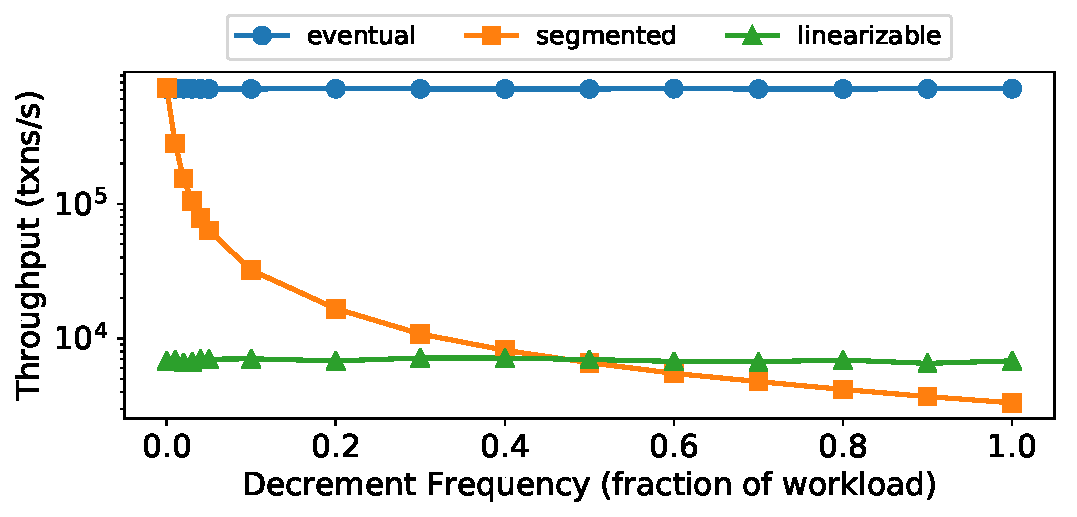
\includegraphics[width=\columnwidth]{figures/vary_withdraws.pdf}
  \end{subfigure}
  \begin{subfigure}[c]{\columnwidth}
    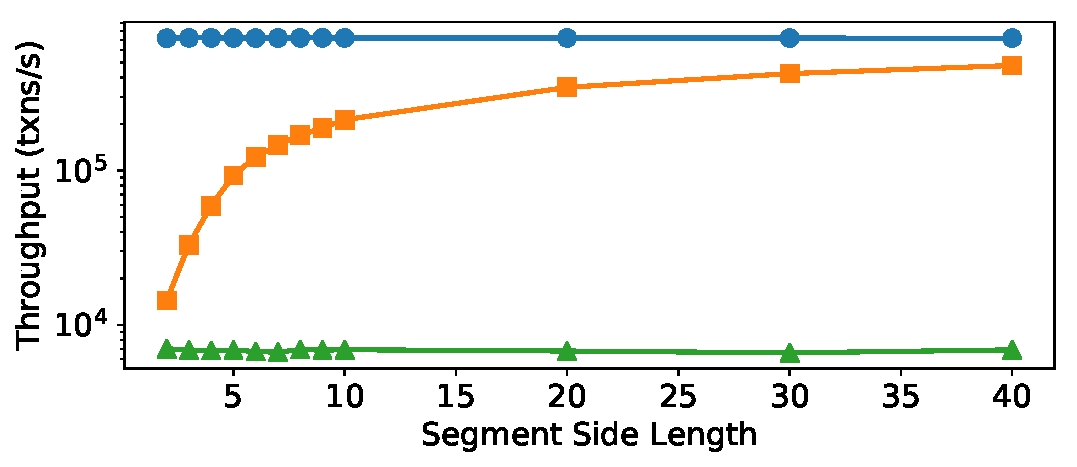
\includegraphics[width=\columnwidth]{figures/vary_segments.pdf}
  \end{subfigure}

  \caption{%
    Segmented invariant-confluent replication throughput versus coordination,
    induced by executing disallowed transactions (top) and by transitioning
    across segments (bottom).
  }\figlabel{ThroughputVsGlobalSyncs}
\end{figure}

\begin{benchmark}\benchlabel{VaryWithdraws}
Consider again the PN-Counter from \exampleref{CounreachableExample} and the
corresponding transactions, invariants, and single-segment segmentation that
forbids concurrent decrements. We replicate this object on 32 servers
deployed on 32 m5.xlarge EC2 instances within the same availability zone.  Each
server has three colocated clients that issue deposit and withdrawal
transactions. We replicate the object with eventual consistency, segmented
invariant-confluence, and linearizability and measure the system's total
throughput as we vary the fraction of client requests that are withdrawals. The
results are shown in the top of \figref{ThroughputVsGlobalSyncs}.

Both eventually consistent replication and linearizable replication are
unaffected by the workload, achieving roughly 700,000 and 7,000 transactions
per second respectively. Expectedly, eventually consistent replication
significantly outperforms linearizable replication because (a) transactions can
be sent to any server (not just the leader) and (b) servers do not coordinate
with each other at all.
%
Segmented invariant-confluent replication performs well for low-withdrawal
workloads and performs increasingly poorly as we increase the fraction of
withdrawal transactions, eventually becoming slower that linearizable
replication. For example, with 5\% withdrawal transactions, segmented
invariant-confluent replication performs an order of magnitude better than
linearizable replication; with 50\% withdrawals, it performs as well; and with
100\% withdrawals, it performs two times worse.

These results are expected. Deposit transactions can execute without any
coordination while withdrawal transactions require global coordination. As we
increase the fraction of withdrawals, we increase the amount of coordination
that the system has to perform which in turn drastically decreases the
throughput. These results also offer two insights:
%
First, for low-withdrawal workloads, segmented invariant-confluent replication
achieves a compromise between strong and weak consistency. It guarantees that
invariants are maintained (which is impossible with eventual consistency if the
object is not invariant-confluent) with performance many times better than
strongly consistent replication.
%
Second, segmented invariant-confluent replication is poorly suited to workloads
that require a large amount of coordination. For workloads without much inherit
concurrency (e.g.\ withdraw-mostly workloads), maintaining invariants is best
done with strong consistency. It provides stronger guarantees with better
performance.
\end{benchmark}

\begin{benchmark}\benchlabel{VarySegmentLength}
  Consider again the object, transactions, and invariants from \exampleref{Z2}
  and \exampleref{SegmentedZ2}. As with \benchref{VaryWithdraws}, we replicate
  the object across 32 servers. Clients issue 50\% increment $x$ transactions,
  and 50\% decrement $y$ transactions. We consider a ``checkerboard''
  segmentation $\Sigma_n = \setst{(I_{i, j}, T)}{i, j \in \ints}$ where segment
  invariant $I_{i, j}$ consists of the square of points $\setst{(x, y)}{ni \leq
  x < n(i + 1), nj \leq y < n(j + 1)}$ with side length $n$. For example,
  $\Sigma_1$ places each point in its own segment, $\Sigma_2$ tessellates
  $\ints^2$ with 2x2 squares, $\Sigma_3$ tessellates $\ints^2$ with 3x3
  squares, and so on. We measure the throughput of the object replicated with
  eventually consistent, segmented invariant-confluent, and linearizable
  replication as we vary the segment side length $n$. The results are shown in
  the bottom \figref{ThroughputVsGlobalSyncs}.

  This benchmark tells the same tale as \benchref{VaryWithdraws}. Eventual
  consistency and linearizability are unaffected by workload, and eventual
  consistency outperforms linearizability by roughly two orders of magnitude.
  In this example, the segmented invariant-confluent replication only requires
  coordination when transitioning between segment boundaries, so as we increase
  the segment side length, the throughput of the system increases
  significantly.
\end{benchmark}

\begin{figure}[ht]
  \centering
  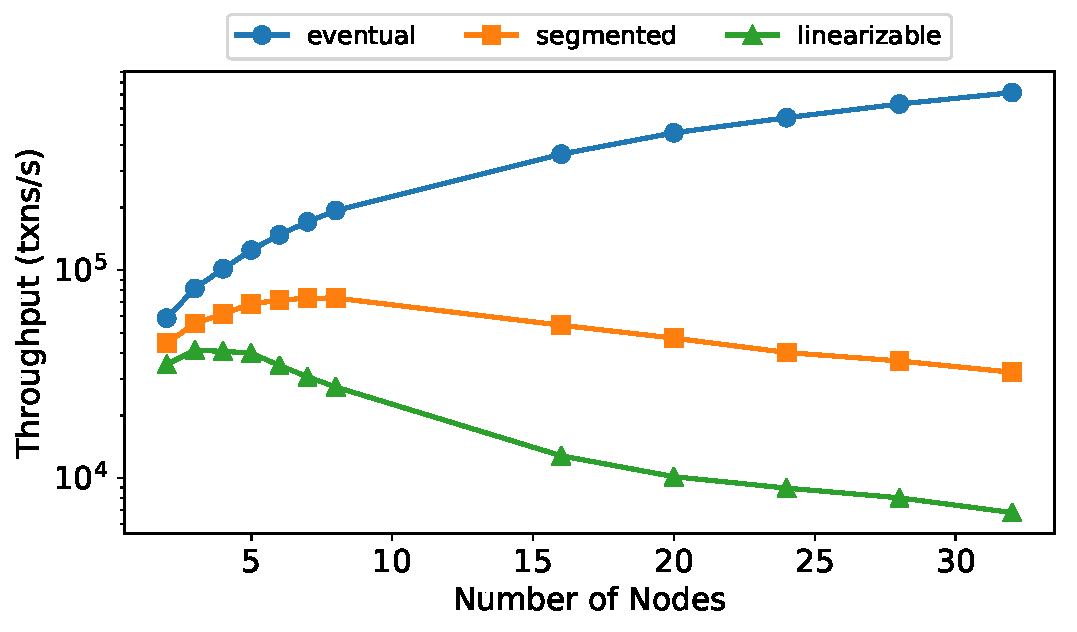
\includegraphics[width=\columnwidth]{figures/vary_nodes.pdf}
  \caption{%
    Throughput of eventually consistent, segmented invariant-confluent, and
    linearizable replication measured against the number of
    nodes.
  }\figlabel{VaryNodes}
\end{figure}

\begin{benchmark}
  In this benchmark, we measure the scale-out of segmented invariant-confluent
  replication. We repeat \benchref{VaryWithdraws} with a 10\% withdrawal rate,
  but this time we vary the number of servers we use to replicate our object.
  When we replicate with $n$ servers, we use $3n$ clients (the $3$ colocated
  clients on each server) as part of the workload. The results are shown in
  \figref{VaryNodes}.

  Eventually consistent replication scales perfectly with the number of nodes,
  confirming the results in~\cite{bailis2014coordination}. With eventually
  consistent replication, servers do not coordinate at all, so they are
  completely unaffected by the number of servers. Linearizable replication, on
  the other hand, scales up to about 3-5 servers before performance begins to
  decrease. These numbers are consistent with typical deployments of
  state-machine replication protocols like Paxos~\cite{chandra2007paxos}.
  Because all messages are sent to the leader, the leader becomes the
  bottleneck as the number of servers and clients increases. Moreover, the
  leader must wait for responses from more servers, increasing the latency of
  the slowest response which in turn decreases throughput.
  Segmented invariant-confluent replication scales up to about 6-8 servers
  before succumbing to the same scalability bottlenecks as linearizable
  replication.

  These results highlight the importance of coordination avoidance in
  distributed databases. While segmented invariant-confluent replication scales
  out slightly better than linearizable replication, both scale significantly
  worse than eventually consistent replication even for a very low (i.e.\ 10\%)
  withdrawal workload. This demonstrates that even a small amount of
  coordination can significantly reduce the scalability of a system.
\end{benchmark}
}
  \bibliography{references}
  \bibliographystyle{plain}
\end{document}
